\section{Pasos de ordenamiento en Excel}
\begin{itemize}[label=$\downarrow$]
    \item Seleccionar todos los datos 
    \item Orden personalizado
    \item Advertencia antes de ordenad $\rightarrow$ Ampliar la selección $\rightarrow$ ordenar 
    \item Ordenar por $\rightarrow$ Valores de celda $\rightarrow$ A a Z
\end{itemize}
%%%%%%%%%%%%%%%%%%%%%%%%%%%%%%%%%%%%%%%%%%%%%%%%%%%%%%%%%%%%%%%%%%%%%%%%%%%%%%%%%%%%%%%%%%%%%%%%
\section{Medidas de localización o tendencia central}   
%%%%%%%%%%%%%%%%%%%%%%%%%%%%%%%%%%%%%%%%%%%%%%%%%%%%%%%%%%%%%%%%%%%%%%%%%%%%%%%%%%%%%%%%%%%%%%%%
\subsection{Media:}
\begin{itemize}
    \item La media aritmética 
    \item La media ponderada
\end{itemize}
\begin{itemize}
    \item La notación que se utilizará sera x-barra:
        \[
            \bar{x} = \frac{\sum_{i=1}^{n}(x_{i})}{n} = \frac{(x_{1} + x_{2} + x_{3} + ... + x_{n})}{n} 
        \]
    
    \item $n$ siendo el número de observaciones.
\end{itemize}
\emph{\textbf{Definición de ``media":} es un número.}
\begin{itemize}
    \item Cuando se agregan valores abnormales al promedio hace un cambio para arriba o para abajo que es significativo.
\end{itemize}

%%%%%%%%%%%%%%%%%%%%%%%%%%%%%%%%%%%%%%%%%%%%%%%%%%%%%%%%%%%%%%%%%%%%%%%%%%%%%%%%%%%%%%%%%%%%%%%%
\subsection{Mediana:}
\begin{itemize}
    \item Es un dato que denota cuánto mide la persona que está cabal en medio.
    \item Es el valor que parte a la mitad todos los datos.
    \item Cuando hay una cantidad impar va a haber uno, cuando es par pueden haber dos.
    \item La mediana no se ve afectada por los valores que están debajo de ella ni arriba de ella.
    \item \[
      \text{Mediana} = \frac{\text{n}}{2} 
    \]
    
    \item Los datos de la media tienen que estar en orden ascendente para poder calcularse.
    \item El número que salga de mediana se usa la parte entera como límite inferior y el número redondeado para arriba es el límite superior, en los números pares.
    \item Si el valor es un número impar se agarra el del medio, si el valor es un numero par se agarra el de floor(enmedio) y el roundedUp(floor(enmedio)).
\end{itemize}

%%%%%%%%%%%%%%%%%%%%%%%%%%%%%%%%%%%%%%%%%%%%%%%%%%%%%%%%%%%%%%%%%%%%%%%%%%%%%%%%%%%%%%%%%%%%%%%%
\subsection{Moda:}
\begin{itemize}
    \item Es el número que más se repite en un set de datos.
    \item No hay fórmula.
\end{itemize}


%%%%%%%%%%%%%%%%%%%%%%%%%%%%%%%%%%%%%%%%%%%%%%%%%%%%%%%%%%%%%%%%%%%%%%%%%%%%%%%%%%%%%%%%%%%%%%%%
\subsection{Percentiles:}
\begin{itemize}
    \item Es un número que nos dice qué porcentaje de los datos esta debajo de él.
    \item La mediana es igual al percentil 50.
    \item Es el límite superior en el cual el porcentaje dicta, el percentil 20 se interpreta como el 20\% de datos están debajo de él.
    \item Percentil:
        \[
          i = \left(\frac{p}{100}  \right) \times n
        \]
        donde $p$ es percentil deseado, e $i$ es el índice.
    
    \item 
        \begin{figure}[htbp]
            \centering
            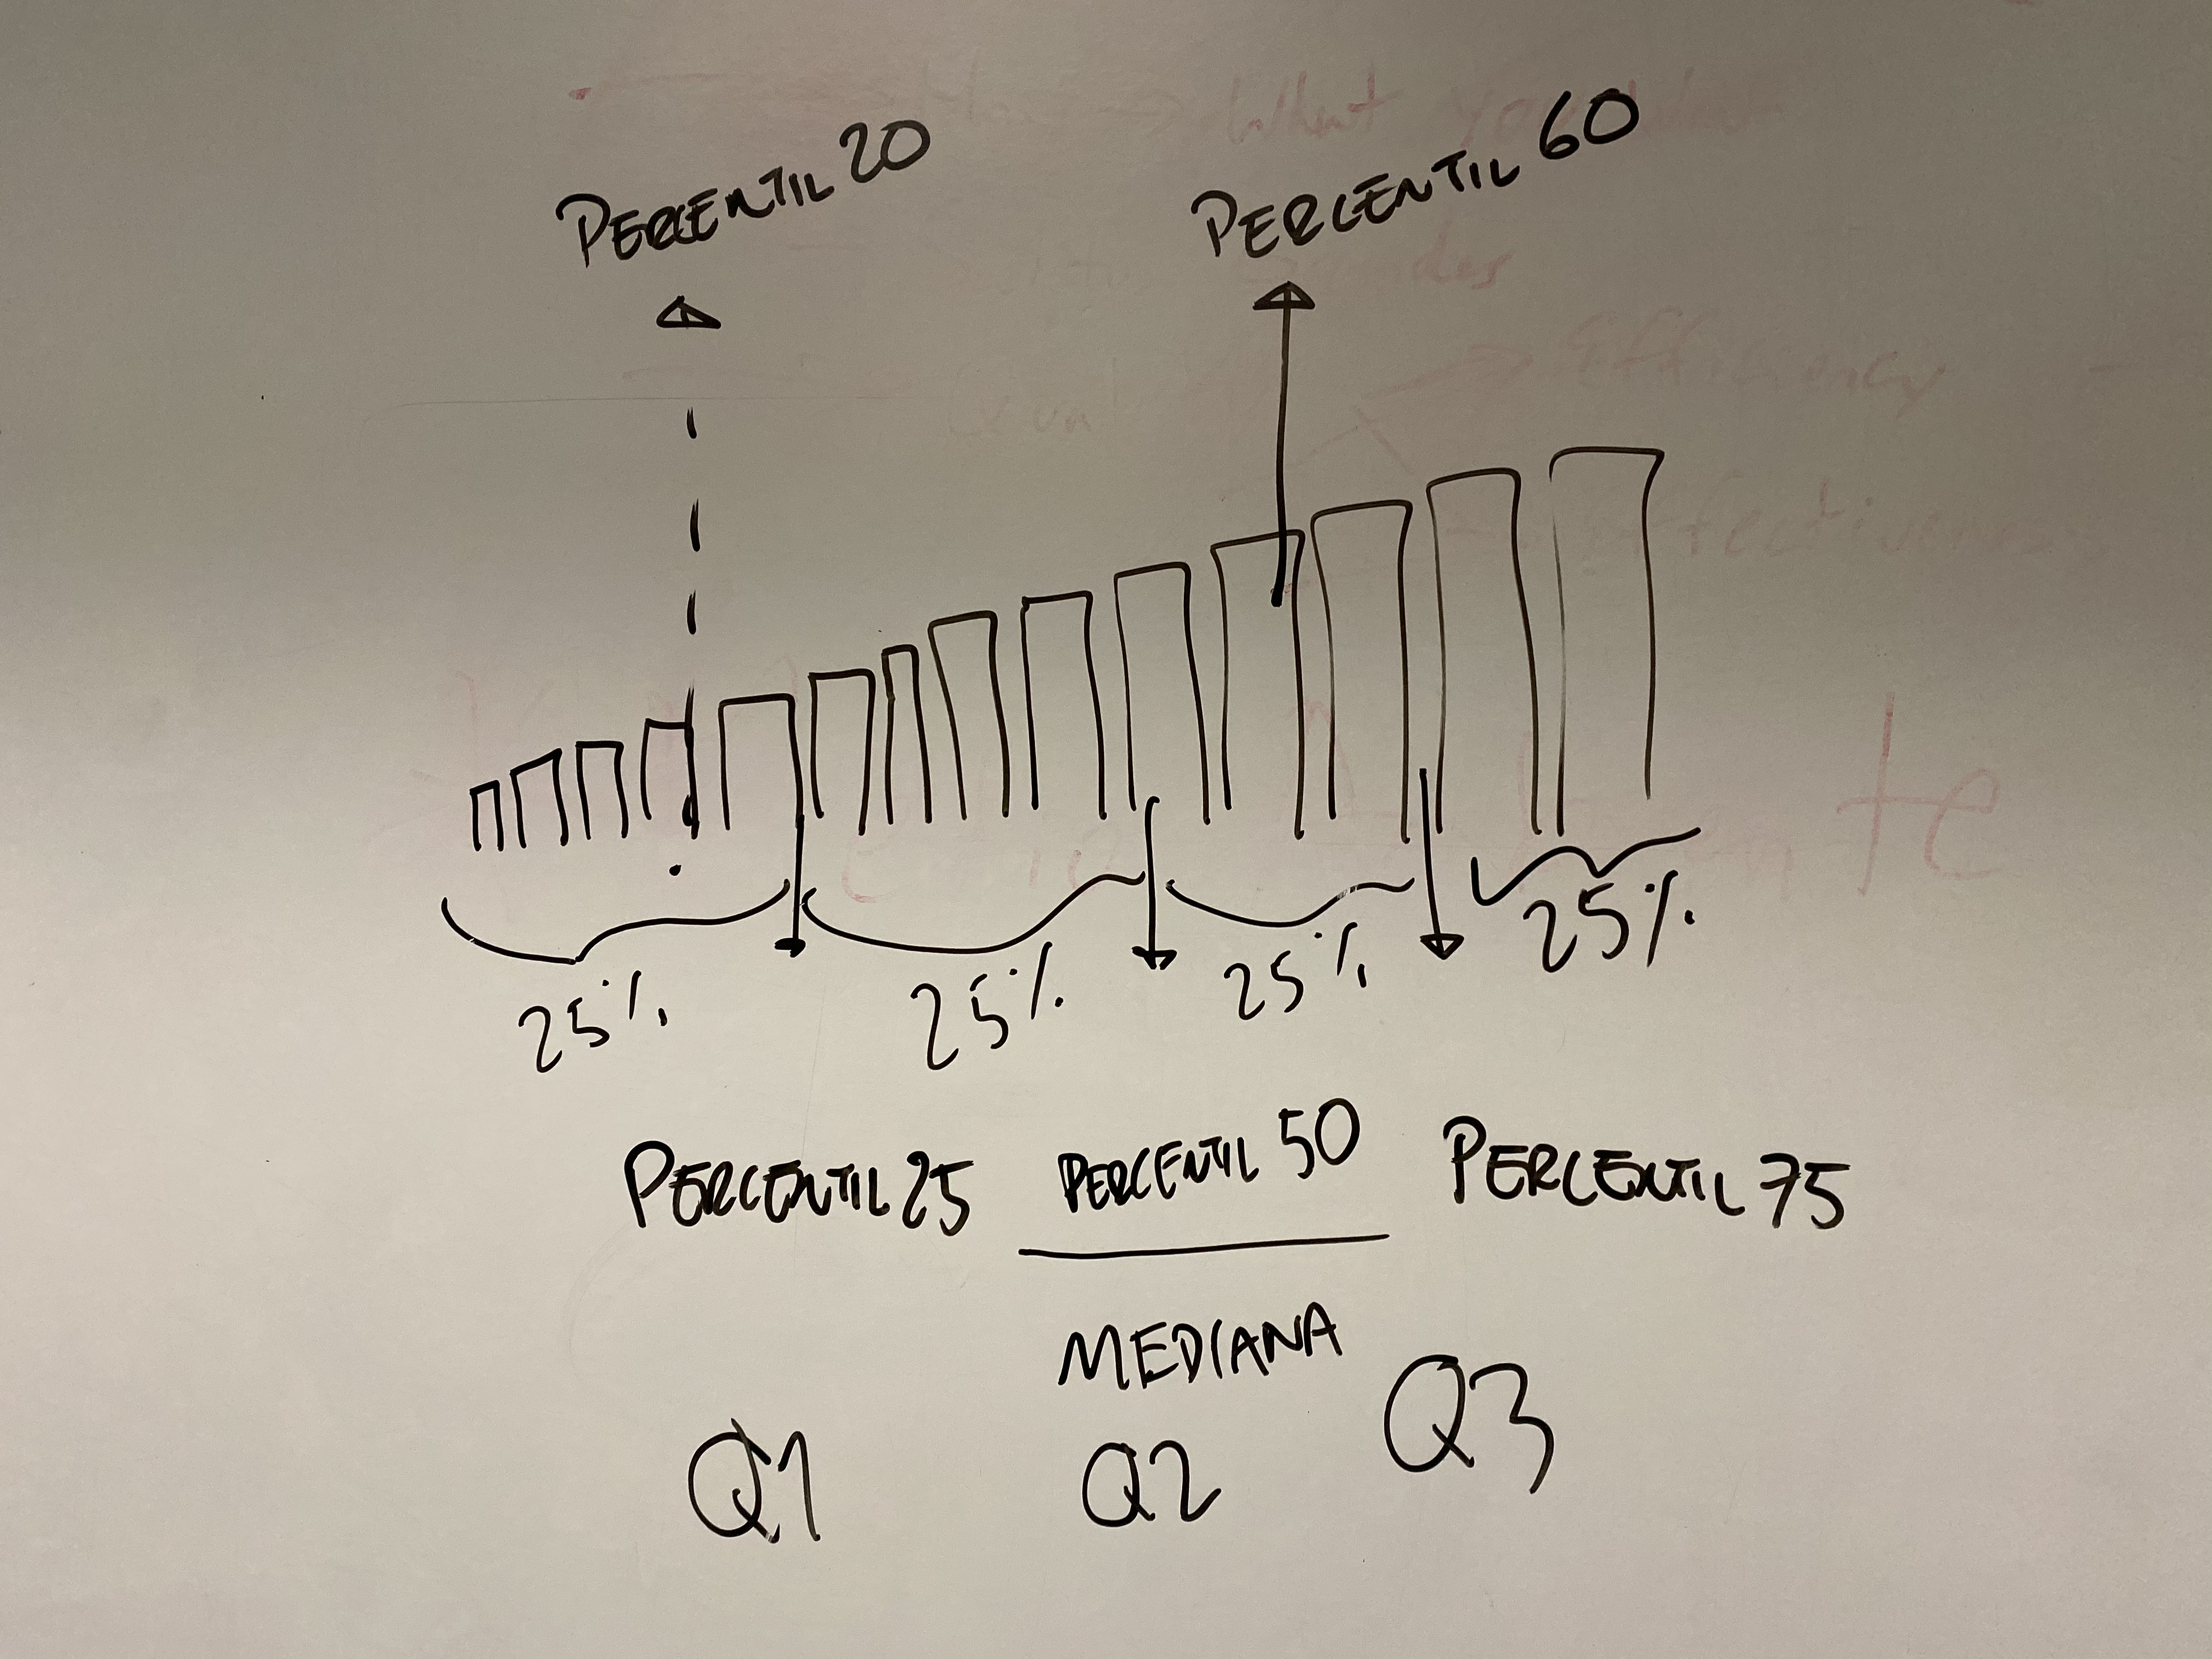
\includegraphics[width=6cm]{Clases/Images/2020-01-14_01.jpeg} 
            \caption{}
            \label{}
        \end{figure} 
\end{itemize}

%%%%%%%%%%%%%%%%%%%%%%%%%%%%%%%%%%%%%%%%%%%%%%%%%%%%%%%%%%%%%%%%%%%%%%%%%%%%%%%%%%%%%%%%%%%%%%%%
\subsection{Cuartiles:}
\begin{itemize}
    \item El cuartil son percentiles partidos en cuatro a lo largo del numero 1-100.
    \item \emph{\textbf{Ejemplo: }El percentil 25\% es el primer cuartil, el 50\% es el segundo cuartil, etcétera.}
\end{itemize}


%%%%%%%%%%%%%%%%%%%%%%%%%%%%%%%%%%%%%%%%%%%%%%%%%%%%%%%%%%%%%%%%%%%%%%%%%%%%%%%%%%%%%%%%%%%%%%%%
\subsection{Observaciones}
\begin{itemize}
    \item \[
      \text{Media} < \text{Mediana} < \text{Moda}  
    \]
        \begin{itemize}
            \item Posiblemente hay más personas de baja estatura, por la media ser menor a la mediana.
        \end{itemize}
    
    \item \[
        \text{Media} > \text{Mediana} > \text{Moda}  
    \]
\end{itemize}
